% I think I need some historical reference here.
Automatic differentiation (AD) is a technology that generates new code representing derivatives of a given parent code. 
Examples are code representing the tangent linear or adjoint operator of the parent code
\cite{Griewank:2008kh}. 
The names \textit{algorithmic} and \textit{computational} differentiation is also used in the literature, emphasizing the algorithmic rather than automatic nature of AD \cite{Griewank:2008kh, Naumann.2011, Margossian_2018}. 
Any computer program implementing a given function can be reduced to a sequence of simple algebraic operations that have straightforward derivative expressions, based upon elementary rules of differentiation \cite{juedes1991taxonomy}.
The derivatives of the outputs of the computer program (dependent variables) with respect to their inputs (independent variables) are then combined using the chain rule.
One advantage of AD systems is their capacity to differentiate complex programs that include control flow, such as branching, loops or recursions. 
% This is because any program can be reduced to a trace of input, intermediate and output variables \cite{Baydin_Pearlmutter_Radul_Siskind_2015}.

AD falls under the category of discrete methods.
Depending on whether the concatenation of the elementary derivatives is done as the program is executed (from input to output) or in a later instance where we trace-back the calculation from the end (from output to input), we refer to \textit{forward} or \textit{reverse} mode AD, respectively.
Neither forward nor reverse mode is more efficient in all cases \cite{Griewank_1989}, as we will discuss in Section \ref{sec:vjp-jvp}.

\subsubsection{Forward mode}

Forward mode AD can be implemented in different ways depending on the data structures we use when representing a computer program. 
Examples of these data structures include dual numbers and computational graphs \cite{Baydin_Pearlmutter_Radul_Siskind_2015}. 
These representations are mathematically equivalent and lead to the same implementation except for details in the compiler optimizations with respect to floating point ordering.

\paragraph{Dual numbers}
\label{section:dual-numbers}

Dual numbers extend the definition of a numerical variable that takes a certain value to also carry information about its derivative with respect to a certain parameter \cite{clifford1871dualnumbers}. 
We define a dual number based on two variables: a \textit{value} coordinate $x_1$ that carries the value of the variable and a \textit{derivative} (also known as partial or tangent) coordinate $x_2$ with the value of the derivative $\frac{\partial x_1}{\partial \theta}$. 
Just as complex number, we can represent dual numbers as an ordered pair $(x_1, x_2)$, sometimes known as Argand pair, or in the rectangular form 
\begin{equation}
 x_\epsilon = x_1 + \epsilon \, x_2,
\end{equation}
where $\epsilon$ is an abstract number called a perturbation or tangent, with the properties $\epsilon^2 = 0$ and $\epsilon \neq 0$.
This last representation is quite convenient since it naturally allow us to extend algebraic operations, like addition and multiplication, to dual numbers \cite{Karczmarczuk2001}. 
For example, given two dual numbers $x_\epsilon = x_1 + \epsilon x_2$ and $y_\epsilon = y_1 + \epsilon y_2$, it is easy to derive, using the fact $\epsilon^2=0$, that
\begin{equation}
 x_\epsilon + y_\epsilon = (x_1 + y_1) + \epsilon \, (x_2 + y_2)
 \qquad
 x_\epsilon y_\epsilon = x_1 y_1 + \epsilon \, (x_1 y_2 + x_2 y_1) .
 %\qquad
 %\frac{x_\epsilon}{y_\epsilon} = \frac{x_1}{y_1} + \epsilon \, \frac{x_2 y_1 - x_1 y_2}{y_1^2}.
\end{equation}
From these last examples, we can see that the derivative component of the dual number carries the information of the derivatives when combining operations.
For example, suppose that in the last example the dual variables $x_2$ and $y_2$ carry the value of the derivative of $x_1$ and $x_2$ with respect to a parameter $\theta$, respectively. 

Intuitively, we can think of $\epsilon$ as being a differential in the Taylor series expansion, as evident in how the output of any scalar functions is extended to a dual number output:
\begin{align}
\begin{split}
    f(x_1 + \epsilon x_2)
    &= 
    f(x_1)
    + 
    \epsilon \, x_2 \,  f'(x_1)
    + 
    \epsilon^2 \cdot ( \ldots )\\
    &= 
    f(x_1)
    + 
    \epsilon \, x_2 \,  f'(x_1).
\end{split}
\label{eq:dual-number-function}
\end{align}
When computing first order derivatives, we can ignore everything of order $\epsilon^2$ or larger, which is represented in the condition $\epsilon^2 = 0$.
This implies that we can use dual numbers to implement forward AD through a numerical algorithm. 
In Section \ref{sec:computational-implementation} we will explore how this is implemented. 

Multidimensional dual number generalize dual number to include a different dual variable $\epsilon_i$ for each variable we want to differentiate with respect to \cite{Neuenhofen_2018, RevelsLubinPapamarkou2016}.
A multidimensional dual number is then defined as $x_\epsilon = x + \sum_{i=1}^p x_i \epsilon_i$, with the property that $\epsilon_i \epsilon_j = 0$ for all pairs $i$ and $j$.
% Notice that a major limitation of the dual number approach is that we need a dual variable for each variable we want to differentiate. 
% This problem can be overcome by computing the full gradient as the combination of independent directional derivatives (see Section \ref{sec:vjp-jvp}). 
Another extension of dual numbers that should not be confused with multidimensional dual numbers are hyper-dual numbers, which allow to compute higher-order derivatives of a function \cite{fike2013multi}. 


\paragraph{Computational graph}
% \vspace*{10px}
% \noindent \textbf{\textit{Computational graph}}
% \vspace*{5px}

A useful way of representing a computer program is via a computational graph with intermediate variables that relate the input and output variables. 
Most scalar functions of interest can be represented as a acyclic directed graph with nodes associated to variables and edges to atomic operations \cite{Griewank:2008kh, Griewank_1989}, known as Kantorovich graph \cite{kantorovich1957mathematical} or its linearized representation via a Wengert trace/tape \cite{Wengert_1964, Bauer_1974, Griewank:2008kh}. 
% Although notation can be a little bit difficult to digest here, the mathematics behind is rather simple. 
We can define $v_{-p+1}, v_{-p+2}, \ldots, v_0 = \theta_1, \theta_2, \ldots, \theta_p$ the input set of variables; $v_{1}, \ldots, v_{m-1}$ the set of all the intermediate variables, and finally $v_m = L(\theta)$ the final output of a computer program. 
This can be done in such a way that the order is strict, meaning that each variable $v_i$ is computed just as a function of the previous variables $v_j$ with $j < i$. 
Once the graph is constructed, we can compute the derivative of every node with respect to the other (a quantity known as the tangent) using the Bauer formula \cite{Bauer_1974, Oktay_randomized-AD}
\begin{equation}
    \frac{\partial v_j}{\partial v_i}
    = 
    \sum_{\substack{ \text{paths }w_0 \rightarrow w_1 \rightarrow \ldots \rightarrow w_K \\
                    \text{with } w_0=v_i, w_K = v_j}}
    \prod_{k=0}^{K-1} \frac{\partial w_{k+1}}{\partial w_{k}},
\end{equation}
where the sum is calculated with respect to all the directed paths in the graph connecting the input and target node.
Instead of evaluating the last expression for all possible paths, a simplification is to increasingly evaluate $j=1, \ldots, m$ using the recursion 
\begin{equation}
    \frac{\partial v_j}{\partial v_i}
    = 
    \sum_\text{$w$\text{ such that} $w \rightarrow v_j$}
    \frac{\partial v_j}{\partial w}
    \frac{\partial w}{\partial v_i} 
    \label{eq:AD-graph-recursion}
\end{equation}
Since every variable node $w$ such that $w \rightarrow v_j$ is an edge of the computational graph has an index less than $j$, we can iterate this procedure as we run the computer program and solve for both the function and its derivative.
This is possible because in forward mode the term $\frac{\partial w}{\partial v_i}$ has been computed in a previous iteration, while $\frac{\partial v_j}{\partial w}$ can be evaluated at the same time the node $v_j$ is computed based on only the value of the parent variable nodes. 
The only requirement for differentiation is being able to compute the derivative/tangent of each edge/primitive and combine these using the recursion defined in Equation \eqref{eq:AD-graph-recursion}.

\subsubsection{Reverse mode}

Reverse mode AD is also known as the adjoint, or cotangent linear mode, or backpropagation in the field of machine learning. 
The reverse mode of automatic differentiation has been introduced in different contexts \cite{griewank2012invented} and materializes the observation made by Phil Wolfe that if the chain rule is implemented in reverse mode, then the ratio between the computational cost of the gradient of a function and the function itself can be bounded by a constant that does not depend on the number of parameters to differentiate \cite{Griewank_1989, Wolfe_1982}, a point known as the \textit{cheap gradient principle} \cite{griewank2012invented}.  
Given a directed graph of operations defined by a Wengert list, we can compute gradients of any given function in the same fashion as Equation \eqref{eq:AD-graph-recursion} but in reverse mode as
\begin{equation}
    \bar v_i 
    = 
    \frac{\partial \ell}{\partial v_i}
    = 
    \sum_\text{$w$\text{ such that} $v_i \rightarrow w$}
    \frac{\partial w}{\partial v_i} \bar{w}.
    \label{eq:reverse-mode-ad-definition}
\end{equation}
In this context, the notation $\bar{w} = \frac{\partial L}{\partial w}$ is introduced to signify the partial derivative of the output variable, here associated to the loss function, with respect to input and intermediate variables. 
This derivative is often referred to as the adjoint, dual, or cotangent, and its connection with the discrete adjoint method will be made more explicitly in Section \ref{section:comparison-discrete-adjoint-AD}. 

Since in reverse-mode AD the values of $\bar w$ are being updated in reverse order, in general
% , i.e., for nonlinear function evaluations or in the presence of complex flow graphs, 
we need to know the state value of all the argument variables $v$ of $w$ in order to evaluate the terms $\frac{\partial w}{\partial v}$.
These state values (required variables) need to be either stored in memory during the evaluation of the function or recomputed on the fly in order to be able to evaluate the derivative. 
Checkpointing schemes exist to limit and balance the amount of storing versus recomputation (see section \ref{section:checkpointing}).


\subsubsection{AD connection with JVPs and VJPs}
\label{sec:vjp-jvp}

When working with unit operations that involve matrix operations dealing with vectors of different dimensions, the order in which we apply the chain rule matters \cite{Giering_Kaminski_1998}.
When computing a gradient using AD, we can encounter vector-Jacobian products (VJPs) or Jacobian-vector products (JVP).
As their name indicates, the difference between them is that the quantity we are interested in is described by the product of a Jacobian times a vector on the left side (VJP) or the right (JVP).
Furthermore, both forward and reverse AD can be thought of as a way of computing derivatives associated with JVPs (see Equation \eqref{eq:directional-derivative}) and VJPs, respectively. 
In other words, given a function $g: \R^{d_1} \mapsto \R^{d_2}$ that is evaluated during the forward mode of given program, AD will carry terms of the form $Dh (x) \cdot \dot x$ (JVP) in forward mode and $\bar y^T \cdot Dh (x)$ (VJP) in reverse mode \cite{Griewank:2008kh}.

Let us consider for example the case of a loss function $L : \mathbb R^p \mapsto \mathbb R$ taking a total of $p$ arguments as inputs that can be decomposed as $L(\theta) = \ell \circ g_{k} \circ \ldots \circ g_2 \circ g_1(\theta)$, with $\ell : \mathbb R^{d_k} \mapsto \mathbb R$ the final evaluation of the loss function after we apply in order a sequence of intermediate functions $g_i : \mathbb R^{d_{i-1}} \mapsto \mathbb R^{d_i}$, where we define $d_0 = p$ for simplicity. 
The final gradient is computed as the chain product of vectors and Jacobians as
\begin{equation}
 \nabla_\theta L = \nabla \ell \cdot Dg_{k} \cdot Dg_{k-1} \cdot \ldots \cdot Dg_2 \cdot Dg_1, 
\end{equation}
% \todo[inline]{Eqn (25) is misleading insofar as it gives the (wrong) impression that grad(L) can be computed in forward mode. But that is not the case. All that can be computed is grad(L)*v(0). The grads should be changed into "D", or you should make the product of grad(L)*v(o) explicit.
% You'll need the transpose of that eqn to get the gradient.}
with $Dg_i$ the Jacobian of each nested function evaluated at the intermediate values $g_{i-1} \circ g_{i-2} \circ \ldots \circ g_i (\theta)$.
Notice that in the last equation $\nabla \ell \in \mathbb R^{d_k}$ is a vector.
% \todo{See above comment: All that eqn (25) can do is solve grad(L)*v(0), ie the directional derivative.}
In order to compute $\nabla_\theta L$, we can solve the multiplication starting from the right side, which will correspond to multiplying the Jacobians forward from $Dg_1$ to $Dg_k$, or from the left side, moving backwards. 
The important aspect of the backwards case is that we will always be computing VJPs, 
% \todo{No, $\nabla \ell$ is not a vector, it's a gradient.}
since $\nabla \ell$ is a vector.
Since VJPs are easier to evaluate than full Jacobians, the reverse mode will in general be faster when $1 \ll p$. This example is illustrated in Figure \ref{fig:vjp-jvp}. 
% \todo[inline]{JVPs are also easier to evaluate than Jacobians. The point is that JVP maps from dim(p) to dim(1), whereas VJP maps from dim(1) to dim(p).}
For general rectangular matrices $A\in \mathbb R^{d_1 \times d_2}$ and $B \in \mathbb R^{d_2 \times d_3}$, the cost of the matrix multiplication $AB$ is $\mathcal O (d_1 d_2 d_3)$.

It is worth noting that while more efficient methods for matrix-matrix multiplication based on Strassen’s recursive algorithm and its variants exist, these are not extensively used in most scientific applications \cite{Silva_Gustafson_Wong_2018, Huang_Smith_Henry_Geijn_2016}.
This implies that forward AD requires a total of
\begin{equation}
 d_2 d_1 p + d_3 d_2 p + \ldots + d_k d_{k-1} p + d_k p = \mathcal O (kp)
\end{equation}
operations, while backwards mode AD requires
\begin{equation}
 d_k d_{k-1} + d_{k-1} d_{k-2} + \ldots + d_2 d_1 + d_1 p = \mathcal O (k+p)
\end{equation}
operations. 

In the general case of a function $L : \R^p \mapsto \R^q$ with multiple outputs and a total of $k$ intermediate functions, the cost of forward AD is $\mathcal O (pk + q)$ and the cost of reverse is $\mathcal O (p + kq)$.
When the function to differentiate has a larger input space than output ($q \ll p$), AD in reverse mode is more efficient as it propagates the chain rule by computing VJPs.
For this reason, reverse-mode AD is preferred in both modern machine learning and inverse methods.
% On the other side, when the output dimension is larger than the input space dimension, forwards AD is more efficient.
% This is the reason why in most machine learning application people use backwards AD. 
However, notice that reverse mode AD requires saving intermediate variables through the forward run in order to run backwards afterwards \cite{Bennett_1973}, leading to performance overhead that makes forward AD more efficient when $p \lesssim q$ \cite{Griewank_1989, Margossian_2018, Baydin_Pearlmutter_Radul_Siskind_2015}. 

\begin{figure}[t]
    \centering
    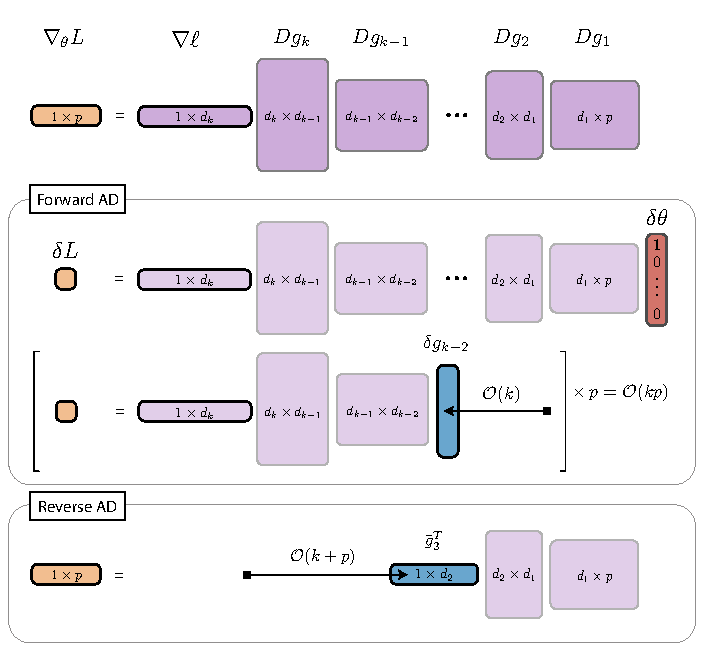
\includegraphics[width=0.95\textwidth]{figures/VJP-AD.pdf}
    \caption{Comparison between forward and reverse mode AD. Changing the order of Jacobian multiplications changes the total number of floating-point operations, which leads to different computational complexities between forward and reverse mode. When the multiplication is carried from the right side of the mathematical expression for $\nabla_\theta L$, each matrix simplification involves a matrix with size $p$, giving a total complexity of $\mathcal O (kp)$. This is the opposite of what happens when we carry the VJP from the left side of the expression, where the matrix of size $d_1 \times p$ has no effect in the intermediate calculations, making all the intermediate calculations $\mathcal O (1)$ with respect to $p$ and a total complexity of $\mathcal O (k + p)$. }
    % However, backwards mode requires storing in memory information about the forward execution of the program, while forward mode can update the gradient on running time.}
    \label{fig:vjp-jvp}
\end{figure}

In practice, many AD systems are reduced to the computation of only directional derivatives (JVPs) or gradients (VJPs) \cite{Griewank:2008kh}.
% An important observation is that most AD systems construct full Jacobians by performing multiple VJPs and JVPs instead of constructing the full Jacobian at once. 
Full Jacobians $J \in \R^{n \times p}$ (e.g., the sensitivity $s = \frac{\partial u}{\partial \theta} \in \R^{n \times p}$) can be fully reconstructed by the independent computation of the $p$ columns of $J$ via the JVPs $J e_i$, with $e_i \in \R^p$ the canonical vectors; or by the calculation of the $m$ rows of $J$ via the VJPs $e_j^T J$, with $e_j \in \R^n$.
Sparse Jacobians are commonplace in large-scale nonlinear systems and discretized PDEs. 
When the sparsity pattern is known, they can be efficiently obtained with \textit{colored AD} to chunk multiple JVPs or VJPs, based on the colored Jacobian~\cite{gebremedhin2005color}.
More concretely, consider the example of a Jacobian, ${J}_{\text{sparse}}$, with known sparsity pattern given by
\begin{equation}
    {J}_{\text{sparse}} = \begin{bmatrix}
        \bullet &         &         &         &         \\
                & \bullet & \bullet &         &         \\
                &         &         & \bullet &         \\
        \bullet & \bullet &         &         & \bullet \\
                &         &         &         & \bullet
    \end{bmatrix},
\end{equation}
where $\bullet$ denotes the non-zero elements of the Jacobian. 
% AD tools compute Jacobians column-wise or row-wise by composing multiple JVPs or VJPs respectively. 
% This is done to avoid perturbation confusion~\cite{manzyuk2019perturbation}. 
We can color the above matrix as follows:
\begin{equation}
    {J}^{(\text{col})}_{\text{sparse}} = \begin{bmatrix}
        \color{myred}{\blacktriangleright} &                            &                                  &                                  &                              \\
                                         & \color{myblue}{\blacksquare} & \color{myred}{\blacktriangleright} &                                  &                              \\
                                         &                            &                                  & \color{myred}{\blacktriangleright} &                              \\
        \color{myred}{\blacktriangleright} & \color{myblue}{\blacksquare} &                                  &                                  & \color{myviolet}{\blacklozenge} \\
                                         &                            &                                  &                                  & \color{myviolet}{\blacklozenge}
    \end{bmatrix} \qquad {J}^{(\text{row})}_{\text{sparse}} = \begin{bmatrix}
        \color{myblue}{\blacksquare}   &                              &                            &                            &                              \\
                                     & \color{myblue}{\blacksquare}   & \color{myblue}{\blacksquare} &                            &                              \\
                                     &                              &                            & \color{myblue}{\blacksquare} &                              \\
        \color{myviolet}{\blacklozenge} & \color{myviolet}{\blacklozenge} &                            &                            & \color{myviolet}{\blacklozenge} \\
                                     &                              &                            &                            & \color{myblue}{\blacksquare}
    \end{bmatrix}.
\end{equation}
To compute $J^{(\text{col})}_{\text{sparse}}$, we just need to perform three JVPs, 
\begin{equation}
    J^{(\text{col})}_{\text{sparse}} 
    \begin{bmatrix}
    1 \\ 0 \\ 1 \\ 1 \\ 0    
    \end{bmatrix}
    = 
    \begin{bmatrix}
    \color{myred}{\blacktriangleright} \\ \color{myred}{\blacktriangleright} \\ \color{myred}{\blacktriangleright} \\ \color{myred}{\blacktriangleright} \\ \\   
    \end{bmatrix}, \qquad
    J^{(\text{col})}_{\text{sparse}} 
    \begin{bmatrix}
    0 \\ 1 \\ 0 \\ 0 \\ 0    
    \end{bmatrix}
    = 
    \begin{bmatrix}
    \\ \color{myblue}{\blacksquare} \\ \\ \color{myblue}{\blacksquare} \\ \\ 
    \end{bmatrix}, \qquad
    J^{(\text{col})}_{\text{sparse}} 
    \begin{bmatrix}
    0 \\ 0 \\ 0 \\ 0 \\ 1    
    \end{bmatrix}
    = 
    \begin{bmatrix}
    \\ \\ \\ \color{myviolet}{\blacklozenge} \\ \color{myviolet}{\blacklozenge} \\ 
    \end{bmatrix},
\end{equation}
compared to five JVPs for a $5 \times 5$ dense Jacobian.
Similarly, since reverse mode materializes the Jacobian one row at a time, we need two VJPs (once each for $\color{myblue}{\blacksquare}$, and $\color{myviolet}{\blacklozenge}$) compared to five VJPs for the dense counterpart. 